
%(BEGIN_QUESTION)
% Copyright 2015, Tony R. Kuphaldt, released under the Creative Commons Attribution License (v 1.0)
% This means you may do almost anything with this work of mine, so long as you give me proper credit

\noindent
{\bf Lab Exercise -- introduction}

\vskip 5pt

Your team's task is to configure an HMI (Human-Machine Interface) for a system controlled by a PLC, as well as add a discrete electrical load and a three-pole contactor (energized by one of the PLC's discrete outputs) to the system.  The HMI you choose to configure shall allow operator access to (at minimum) discrete input data points, discrete output data points, and either counter or timer instructions.  Project ideas include:

\begin{itemize}
\item{} Air compressor control, with high and low air pressure switches
\vskip 5pt
\item{} Water sump pump control, with high and low water level switches
\vskip 5pt
\item{} Other alternatives? {\it Must be pre-approved by instructor!}
\end{itemize}

The following table of objectives show what you and your team must complete within the scheduled time for this lab exercise.  Note how some of these objectives are individual, while others are for the team as a whole:

\vskip 10pt

\underbar{Objective completion table:}

% No blank lines allowed between lines of an \halign structure!
% I use comments (%) instead, so that TeX doesn't choke.

$$\vbox{\offinterlineskip
\halign{\strut
\vrule \quad\hfil # \ \hfil & 
\vrule \quad\hfil # \ \hfil & 
\vrule \quad\hfil # \ \hfil & 
\vrule \quad\hfil # \ \hfil & 
\vrule \quad\hfil # \ \hfil & 
\vrule \quad\hfil # \ \hfil & 
\vrule \quad\hfil # \ \hfil \vrule \cr
\noalign{\hrule}
%
% First row
{\bf Performance objective} & {\bf Grading} & {\bf 1} & {\bf 2} & {\bf 3} & {\bf 4} & {\bf Team} \cr
%
\noalign{\hrule}
%
% Another row
Team meeting and prototype sketch (do {\it first!}) & mastery & -- & -- & -- & -- & \cr
%
\noalign{\hrule}
%
% Another row
Circuit design challenge & mastery & & & & & -- -- -- -- \cr
%
\noalign{\hrule}
%
% Another row
Final tagname database for HMI & mastery & -- & -- & -- & -- & \cr
%
\noalign{\hrule}
%
% Another row
Final wiring diagram and system inspection & mastery & & & & & -- -- -- -- \cr
%
\noalign{\hrule}
%
% Another row
Demonstration of working system & mastery & -- & -- & -- & -- & \cr
%
\noalign{\hrule}
%
% Another row
Final PLC program inspection & mastery &  &  &  &  & -- -- -- --  \cr
%
\noalign{\hrule}
%
% Another row
Troubleshooting & mastery & & & & & -- -- -- -- \cr
%
\noalign{\hrule}
%
% Another row
Lab question: Wiring connections & proportional &  &  &  &  & -- -- -- -- \cr
%
\noalign{\hrule}
%
% Another row
Lab question: Commissioning & proportional &  &  &  &  & -- -- -- -- \cr
%
\noalign{\hrule}
%
% Another row
Lab question: Mental math & proportional &  &  &  &  & -- -- -- -- \cr
%
\noalign{\hrule}
%
% Another row
Lab question: Diagnostics & proportional &  &  &  &  & -- -- -- -- \cr
%
\noalign{\hrule}
%
% Another row
Decommission and lab clean-up & mastery & -- & -- & -- & -- &  \cr
%
\noalign{\hrule}
%
% Another row
Team tool locker inspection & mastery & -- & -- & -- & -- &  \cr
%
\noalign{\hrule}
} % End of \halign 
}$$ % End of \vbox

The only ``proportional'' scoring in this activity are the lab questions, which are answered by each student individually.  A listing of potential lab questions are shown at the end of this worksheet question.  The lab questions are intended to guide your labwork as much as they are intended to measure your comprehension, and as such the instructor may ask these questions of your team day by day, rather than all at once (on a single day).

\vskip 10pt

{\bf It is essential that your team plans ahead what to accomplish each day.  A short (10 minute) team meeting at the beginning of each lab session is a good way to do this, reviewing what's already been done, what's left to do, and what assessments you should be ready for.  There is a lot of work involved with building, documenting, and troubleshooting these working instrument systems!}

As you and your team work on this system, you will invariably encounter problems.  You should always attempt to solve these problems as a team before requesting instructor assistance.  If you still require instructor assistance, write your team's color on the lab whiteboard with a brief description of what you need help on.  The instructor will meet with each team in order they appear on the whiteboard to address these problems.





\vfil \eject

\noindent
{\bf Lab Exercise -- team meeting and prototype sketch}

\vskip 5pt

An important first step in completing this lab exercise is to {\bf meet with your instructor} as a team to discuss safety concerns, team performance, and specific roles for team members.  If you would like to emphasize exposure to certain equipment (e.g. use a particular type of control system, certain power tools), techniques (e.g. fabrication), or tasks to improve your skill set, this is the time to make requests of your team so that your learning during this project will be maximized.

\vskip 10pt

An absolutely essential step in completing this lab exercise is to work together as a team to {\bf sketch a prototype diagram} showing what you intend to build.  This usually takes the form of a simple electrical schematic and/or loop diagram showing all electrical connections between components, as well as any tubing or piping for fluids.  This prototype sketch need not be exhaustive in detail, but it does need to show enough detail for the instructor to determine if all components will be correctly connected for their safe function.

For example, if you intend to connect field devices to a PLC (Programmable Logic Controller), your prototype sketch must show how those devices will connect to typical input/output terminals on the PLC, where electrical power will be supplied, etc.  Prototype sketches need not show all intermediary connections between components, such as terminal blocks in junction boxes between the field device and the controller.

You should practice good problem-solving techniques when creating your prototype sketch, such as consulting equipment manuals for information on component functions and marking directions of electric current, voltage polarities, and identifying electrical sources/loads.  Use this task as an opportunity to strengthen your analytical skills!  Remember that you will be challenged in this program to do all of this on your own (during ``capstone'' assessments), so do not make the mistake of relying on your teammates to figure this out for you -- instead, treat this as a problem {\it you} must solve and compare your results with those of your teammates.

Your team's prototype sketch is so important that the instructor will demand you provide this plan before any construction on your team's working system begins.  {\it Any team found constructing their system without a verified plan will be ordered to cease construction and not resume until a prototype plan has been drafted and approved!}  Similarly, you should not deviate from the prototype design without instructor approval, to ensure nothing will be done to harm equipment by way of incorrect connections.  Each member on the team should have ready access to this plan (ideally possessing their own copy of the plan) throughout the construction process.  Prototype design sketching is a skill and a habit you should cultivate in school and take with you in your new career.

\vskip 10pt

When selecting a three-pole contactor to include in this project, choose one with a coil compatible with the discrete outputs of your PLC.  If your PLC's discrete outputs are a mis-match for the contactor coil, you will need to install an {\it interposing relay} to convert the PLC's DC output control signal into a driving signal suitable for the contactor (e.g. a relay interposing between a PLC with 24 VDC discrete outputs and a contactor with a 120 VAC rated coil).

PLC equipment manuals always provide sample diagrams showing how external components may connect to the I/O points.  Feel free to use these sample diagrams as templates for your prototype sketch.  {\it This is the most challenging portion of your wiring, so be sure to work with your teammates to get this right!}

\vskip 10pt

{\bf Planning a functioning system should take no more than a couple of hours if the team is working efficiently, and will save you hours of frustration (and possible component destruction!).}








\vfil \eject

\noindent
{\bf Lab Exercise -- planning the interface}

\vskip 5pt

An essential step in programming an HMI panel is to define the list of {\it tagnames} and {\it data types} the HMI will need to reference in order to fulfill its function.  While this seems like something that may be done while in the process of programming the HMI's graphical display objects, it is actually best done {\it before} any HMI programming is done at all.  Listing all the signals and variables the HMI will need to reference within the PLC it connects to as a first step helps ensure that the naming convention you choose for these tags make sense in the grand scheme of the system design, rather than being ad-hoc in nature.  Well-named tags go a long way to making the HMI easier to understand and update in the future.  It also helps identify changes that may need to be made to the PLC program to provide the HMI with all the data it will need.

\vskip 10pt

The next step should be finding appropriate documentation for your HMI.  You may locate this on the HMI manufacturer's website.  Use this documentation to identify how to properly wire, power, and program the HMI display unit.

\vskip 10pt

{\bf Planning the interface should take no more than an hour if the team is working efficiently, and will save you hours of frustration (and possible component destruction!).}






\vfil \eject

\noindent
{\bf Lab Exercise -- circuit design challenge}

\vskip 5pt

Your instructor will choose one VFD or discrete sensing device and one brand/model of PLC from the lists shown below, for which you must sketch an accurate circuit diagram showing how the PLC would connect to the VFD or sensor control/receive its status.  If additional electrical components are required (e.g. DC power source, electromechanical relay, etc.), those must be incorporated into your diagram as well.  Instruction manuals for all devices listed are available on the electronic Instrumentation Reference for your convenience.  When your sketch is complete, you must show the relevant manual pages to your instructor for verification of correct connections.

This exercise tests your ability to locate appropriate information in technical manuals and sketch a correct discrete control circuit for a given PLC and sensor/VFD.  The electronic Instrumentation Reference will be available to you in order to answer this question.

\vskip 10pt

It is highly recommended that you approach this exercise the same as for the design of any other electrical circuit: carefully identify all {\it sources} and {\it loads} in the circuit, identify devices requiring DC versus devices requiring AC, trace directions of all currents (DC only), and mark the polarities of all voltages (DC only).  Most of the mistakes made in this type of circuit design challenge may be remedied by careful consideration of these specific circuit-analysis details.



%%%%%%%%%%%%%%%%%%%%%%%%%%%%%%%
\vskip 10pt
\filbreak
\hbox{ \vrule
\vbox{ \hrule \vskip 3pt
\hbox{ \hskip 3pt
\vbox{ \hsize=5in \raggedright

\noindent \centerline{\bf Switch options}
\begin{itemize}
\item{} Proximity/limit switch
\begin{itemize}

\item{} Mechanical process switch with form-C contacts
\item{} Inductive proximity switch, sourcing
\item{} Inductive proximity switch, sinking
\end{itemize}
\vskip 2pt
\item{} Level
\begin{itemize}

\item{} Rosemount 2120 vibrating fork level switch with PNP output
\end{itemize}
\end{itemize}

} \hskip 3pt}%
\vskip 5pt \hrule}%
\vrule}
%%%%%%%%%%%%%%%%%%%%%%%%%%%%%%%



%%%%%%%%%%%%%%%%%%%%%%%%%%%%%%%
\vskip 10pt
\filbreak
\hbox{ \vrule
\vbox{ \hrule \vskip 3pt
\hbox{ \hskip 3pt
\vbox{ \hsize=5in \raggedright

\noindent \centerline{\bf PLC options}
\begin{itemize}
\item{} Siemens S7-300 I/O cards
\begin{itemize}

\item{} Input module: DI 32 x DC 24 V (6ES7321-1BL00-0AA0)
\item{} Input module: DI 16 x DC 24 V (6ES7321-1BH50-0AA0)
\item{} Input module: DI 16 x DC 48-125 V (6ES7321-1CH20-0AA0)
\item{} Output module: DO 32 x AC 120/230 V/1A (6ES7322-1FL00-0AA0)
\item{} Output module: DO 16 x DC 24 V/0.5A (6ES7322-1BH01-0AA0)
\item{} Output module: DO 16 x Rel (6ES7322-1HH01-0AA0)
\end{itemize}
\vskip 2pt
\item{} Rockwell (Allen-Bradley) ControlLogix 5000 I/O cards
\begin{itemize}

\item{} Input module: 1756-IB16 (16-channel discrete 24 VDC)
\item{} Output module: 1756-OA8 (8-channel discrete 120 VAC)
\item{} Output module: 1756-OB8 (8-channel discrete 24 VDC)
\item{} Output module: 1756-OW16I (16-channel discrete relay)
\end{itemize}
\end{itemize}

} \hskip 3pt}%
\vskip 5pt \hrule}%
\vrule}
%%%%%%%%%%%%%%%%%%%%%%%%%%%%%%%




%%%%%%%%%%%%%%%%%%%%%%%%%%%%%%%
\vskip 10pt
\filbreak
\hbox{ \vrule
\vbox{ \hrule \vskip 3pt
\hbox{ \hskip 3pt
\vbox{ \hsize=5in \raggedright

\noindent \centerline{\bf VFD options}
\begin{itemize}
\item{} Rockwell PowerFlex 4 (discrete ``run'' input in SNK mode)
\item{} Rockwell PowerFlex 4 (discrete ``run'' input in SRC mode)
\item{} Automation Direct GS1 (discrete ``forward'' input)
\end{itemize}

} \hskip 3pt}%
\vskip 5pt \hrule}%
\vrule}
%%%%%%%%%%%%%%%%%%%%%%%%%%%%%%%

\vskip 10pt

Note: a very effective problem-solving strategy for determining how to connect different electrical components together to create a DC circuit is to first identify whether each component acts as a {\it source} or a {\it load} in that circuit.  Then, label voltage polarities (+ , $-$) and directions of current accordingly.  Knowing which way current must flow through each component and which polarity each voltage must have is key to ensuring the inter-component connections are correct.





\vfil



\vfil \eject

\noindent
{\bf Lab Exercise -- documenting the system}

\vskip 5pt

Since this lab exercise involves the inclusion of a three-pole electrical contactor and load, you may have to modify your wiring diagram from the previous lab exercise.  The same standards from the last lab exercise apply here: it must show every connection, every cable, every terminal block, etc.  

When your entire team is finished updating your individual wiring diagrams, call the instructor to do an inspection of the system.  Here, the instructor will have students take turns going through the entire system, with the other students checking their diagrams for errors and omissions along the way.  During this time the instructor will also inspect the quality of the installation, identifying problems such as frayed wires, improperly crimped terminals, poor cable routing, missing labels, lack of wire duct covers, etc.  The team must correct all identified errors in order to receive credit for their system.  

After successfully passing the inspection, each team member needs to place their wiring diagram in the diagram holder located in the middle of the lab behind the main control panel.  When it comes time to troubleshoot another team's system, this is where you will go to find a wiring diagram for that system!

\vskip 10pt







\vfil \eject

\noindent
{\bf Lab Exercise -- troubleshooting}

\vskip 5pt

The most challenging aspect of this lab exercise is {\it troubleshooting}, where you demonstrate your ability to logically isolate a problem in the system.  All troubleshooting is done on an individual basis (no team credit!), and must be done {\it on a system you did not help build}, so that you must rely on loop diagrams to find your way around the system instead of from your own memory of building it.

Each student is given a limited amount of time to identify both the general location and nature of the fault, logically justifying all diagnostic steps taken.  All troubleshooting activities will take place under direct instructor supervision to ensure students are working independently and efficiently. 

Failure to correctly identify both the general location and nature of the fault within the allotted time, and/or failing to demonstrate rational diagnostic procedure to the supervising instructor will disqualify the effort, in which case the student must re-try with a different fault.  Multiple re-tries are permitted with no reduction in grade.

A standard multimeter is the only test equipment allowed during the time limit.  No diagnostic circuit breaks are allowed except by instructor permission, and then only after correctly explaining what trouble this could cause in a real system.  

The instructor will review each troubleshooting effort after completion, highlighting good and bad points for the purpose of learning.  Troubleshooting is a skill born of practice and failure, so do not be disappointed in yourself if you must make multiple attempts to pass!  One of the important life-lessons embedded in this activity is how to deal with failure, because it {\it will} eventually happen to you on the job!  There is no dishonor in failing to properly diagnose a fault after doing your level best.  The only dishonor is in taking shortcuts or in giving up.

\vskip 10pt

{\bf Common mistakes:}

\begin{itemize}
\item{} Neglecting to take measurements with your multimeter.
\item{} Neglecting to check other measurements in the system (e.g. pressure gauge readings).
\item{} Incorrectly interpreting the loop diagram (e.g. thinking you're at the wrong place in the system when taking measurements).
\item{} Incorrect multimeter usage (e.g. AC rather than DC, wrong range, wrong test lead placement).  This is especially true when a student comes to lab unprepared and must borrow someone else's meter that is different from theirs!
\end{itemize}

\vskip 10pt

{\bf Remember that the purpose of the troubleshooting exercise is to foster and assess your ability to intelligently diagnose a complex system.  Finding the fault by luck, or by trial-and-error inspection, is not a successful demonstration of skill.  The only thing that counts as competence is your demonstrated ability to logically analyze and isolate the problem, correctly explaining all your steps!}

\vskip 10pt

{\bf Troubleshooting takes a lot of lab time, usually at least two 3-hour lab sessions for everyone in a full class to successfully pass.  Be sure your team budgets for this amount of time as you plan your work, and also be sure to take advantage of your freedom to observe others as they troubleshoot, to better learn this art.}







\vfil \eject

\noindent
\underbar{Lab Questions} 

\begin{itemize}
\item{} {\bf Wiring connections}
\item{} Determine correct wire connections between field components and a PLC I/O card to create a working PLC input or output circuit, based on diagrams of components with terminals labeled
\item{} Correctly determine all electrical sources and loads, as well as all voltage polarities and current directions in a DC input or output circuit, based on diagrams of field components and the PLC's I/O card with terminals labeled
\end{itemize}

\filbreak

\begin{itemize}
\item{} {\bf Commissioning and Documentation}
\item{} Explain what a ``boolean'' data point is in a PLC or an HMI 
\item{} Explain what an ``integer'' data point is in a PLC or an HMI 
\item{} Explain what a ``fixed point'' data point is in a PLC or an HMI 
\item{} Explain what a ``floating point'' data point is in a PLC or an HMI 
\item{} Explain what an  ``ASCII'' data point is in a PLC or an HMI 
\end{itemize}

\filbreak

\begin{itemize}
\item{} {\bf Mental math} (no calculator allowed!)
\item{} Convert a binary number into decimal
\item{} Convert a binary number into hexadecimal
\item{} Convert a decimal number into binary
\item{} Convert a hexadecimal number into binary
\item{} Convert a hexadecimal number into decimal
\end{itemize}

\filbreak

\begin{itemize}
\item{} {\bf Diagnostics}
\item{} Examine a PLC program and identify any mistakes in it
\item{} Determine whether or not a given diagnostic test will provide useful information, given a set of symptoms exhibited by a failed system
\item{} Identify at least two plausible faults given the results of a diagnostic test and a set of symptoms exhibited by a failed system
\item{} Propose a diagnostic test for troubleshooting a failed system and then explain the meanings of two different test results
\end{itemize}


\underbar{file i03741}
%(END_QUESTION)





%(BEGIN_ANSWER)


%(END_ANSWER)





%(BEGIN_NOTES)

\noindent
{\bf Wiring diagrams / inspections:}

I strongly recommend checking off students' wiring diagrams while you inspect their circuit (checking for secure wiring, proper tubing, good conduit installation, etc.) with them.  Have all team members take you on a ``tour'' of their completed system, with each team member explaining a different portion of the circuit you select while using their own wiring diagram as a guide.  While a student is explaining their section of the system, you can check the other students' wiring diagrams for accuracy.  This not only saves time by consolidating the tasks of system inspection and wiring diagram verification, but it also ensures students can actually relate their wiring diagrams to the system they have built and articulate that understanding to you.

\vskip 10pt

\goodbreak

\noindent
{\bf Troubleshooting fault ideas:}

The turbocompressor system in the lab makes an excellent platform for PLC troubleshooting:

\begin{itemize}
\goodbreak
\item{} Place PLC processor in ``Program'' mode
\item{} Force input or output bits in the PLC
\item{} Pull power fuse
\item{} Shut off valve somewhere (e.g. isolation valve on oil pressure switch)
\item{} Switch NO/NC wiring on one of the pushbutton switches (construction fault)
\item{} Strip wire at terminal, then insert insulated wire end under terminal and tighten (open wire fault)
\item{} Cut signal cable somewhere in mid-conduit (open wire fault)
\item{} Push a thumbtack through the cable somewhere in mid-conduit (shorted wire fault)
\item{} Plug air tube connections using portion of foam earplug stuffed into tube fitting (slow response fault)
\end{itemize}











\vfil \eject

\noindent
{\bf Lab questions}

\vskip 20pt

\item{$(1)$} Sketch all necessary wire connections so that PLC input {\tt I/0} will energize for any pressure condition greater than 10 PSI.  Assume the input channels on this PLC are built to {\it sink} current:

$$\includegraphics[width=15.5cm]{i03741x01.eps}$$

\vskip 20pt

\item{$(2)$} Explain what a ``floating point'' data point is in a PLC or an HMI. 

\vskip 20pt

\item{$(3)$} Convert 96 (decimal) into binary.

\vskip 20pt

\filbreak

\item{$(4)$} An elevator is used at a facility to transport people and equipment between the ground floor and an second floor.  A pair of limit switches sense when the elevator platform reaches each floor position, to tell the PLC when to stop moving the platform.  The PLC control system has a problem, though: the elevator is stuck on the ground floor and refuses to go up.  With no pushbuttons pressed, you examine the I/O card LED indicators and see only three lit: input channels {\tt IN1}, {\tt IN2}, and {\tt IN5}.  Identify one specific fault which could account for all the symptoms, as well as one specific component in this system which is definitely not to blame.  Be sure to specify your proposed fault as either being ``open'' or ``shorted'': 

$$\includegraphics[width=15.5cm]{i03741x02.eps}$$











\vfil \eject

\noindent
{\bf Lab questions}

\vskip 20pt

\item{$(1)$} Sketch all necessary wire connections so that PLC input {\tt I/1} will energize for any pressure condition less than 55 PSI.  Assume the input channels on this PLC are built to {\it source} current:

$$\includegraphics[width=15.5cm]{i03741x01.eps}$$

\vskip 20pt

\item{$(2)$} Explain what an ``integer'' data point is in a PLC or an HMI.

\vskip 20pt

\item{$(3)$} Convert 125 (decimal) into hexadecimal.

\vskip 20pt

\filbreak

\item{$(4)$} An elevator is used at a facility to transport people and equipment between the ground floor and an second floor.  A pair of limit switches sense when the elevator platform reaches each floor position, to tell the PLC when to stop moving the platform.  The PLC control system has a problem, though: the elevator is stuck in mid-position between the two floors and refuses to move either up or down.  With no pushbuttons pressed, you examine the I/O card LED indicators and see only one lit: input channel {\tt IN5}.  Identify one specific fault which could account for all the symptoms, as well as one specific component in this system which is definitely not to blame.  Be sure to specify your proposed fault as either being ``open'' or ``shorted'': 

$$\includegraphics[width=15.5cm]{i03741x02.eps}$$

%INDEX% Lab exercise, HMI configuration for PLC-controlled system

%(END_NOTES)


